\subsection{Kullback Leibler Divergence}

\subsubsection{The formula}
The \emph{Kullback-Leibler} (KL) Divergence is not, as its name indicates it, a mesure of a distance between subsets of the corpus, but it s a divergence between them. Indeed, let us consider to set $P$ and $Q$ containing articles for one year each. The KL divergence is defined as follows :

\begin{eqnarray}\label{KL}
    D_{KL}(P||Q) = \sum_i P(i) ln \frac{P(i)}{Q(i)}
\end{eqnarray}

It computes the sum of multiplications between the probability of the word $i$ in corpus $P$ and the natural logarithm of the same probability over the probability of the word $i$ in $Q$. Thus, $P$ and $Q$ need to be arrays containing the same words at the same indexes. We also can explain the \emph{Kullback-Leibler} Divergence as the lost when $Q$ is used to approximate $P$ or, in other words, as the fact that $Q$ tries to simulate $P$.

Obviously, this divergence is not symmetric. Indeed, let us take for example two years $y_1$ and $y_2$ from the corpus. Suppose now that $y_1$ contains more common words than $y_2$, that contains more uncommon words. We can conclude that $y_2$ will simulate $y_1$ than $y_1$ will simulate $y_2$. This is only because $y_2$ has a bigger subset of words of $y_1$, so it can simulate it easily. We can observe this phenomenon in the following graphs. The years around 1840 have some difficulties to simulate 1990's years but in the other direction it is easy because there is more vocabulary in the 20th century than in the 19th.\\

To compute this formula, as we need to have vectors with the same size representing the same words in the same order and as some words appear only in certain year, it is mandatory to add the missing words in each year with a number of occurrences equal to 0. Doing so, we have for each year a vector containing all words over the whole corpus. With KL Divergence, we have to be careful, because if $P(i)$ or $Q(i)$ is 0, the computation will be totally wrong. Thus, we have to add some smoothing in the KL computation. We made the choice to add a really small value ($10^{_25}$) and to weight it with the probability of the word over the whole corpus. Thus, we keep a small difference between words that appear a lot in the corpus and the one that appear not so much\footnote{It is a way to have less consideration for word that appear not so much, like words that are not in french and that we not be able to correct perfectly.}.

\subsubsection{Computation of \emph{Kullback-Leibler} Divergence}
We computed the \emph{Kullback-Leibler} Divergence with the non-corrected corpus and the OCR-corrected corpus and using the probability that a word appear in a year and the TF-IDF value of each word. The explanations about the graphs are located below.

\begin{figure}[h!]
    \begin{minipage}[b]{0.48\linewidth}
        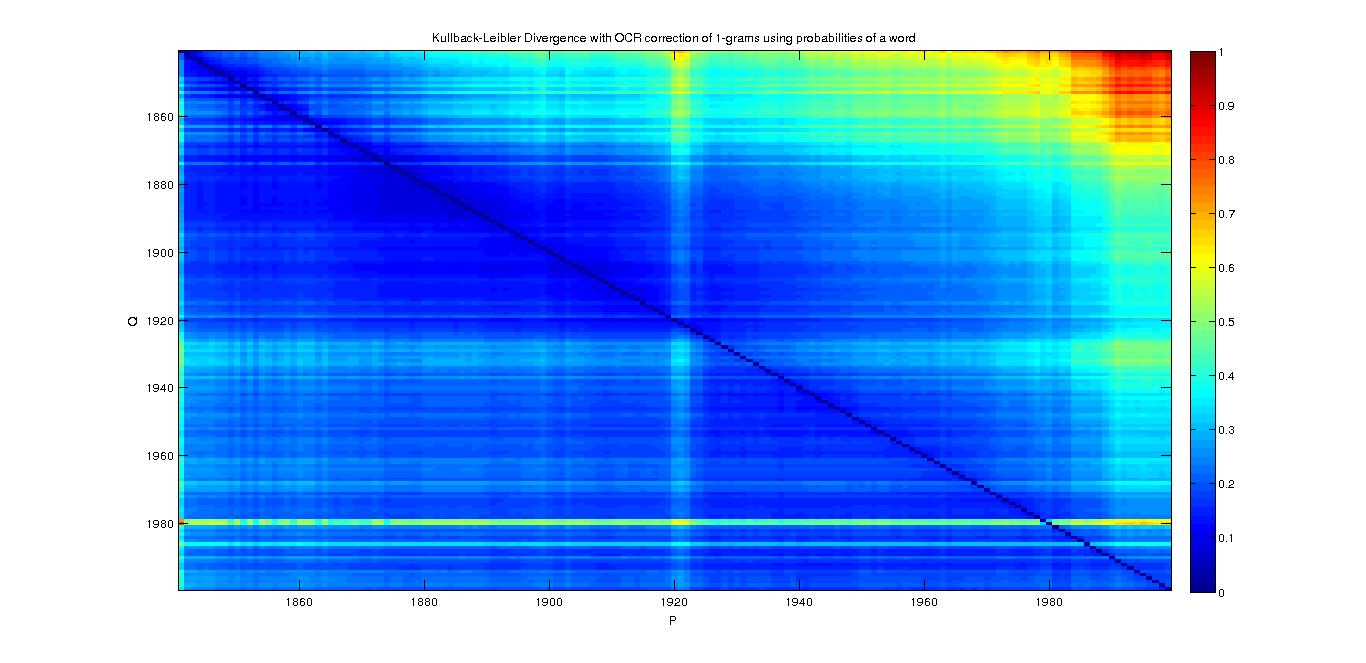
\includegraphics[scale=0.15]{Pictures/kullback-leibler/KL_1-grams_with_correction_proba.jpg}
        \caption{KL for 1-gram with OCR correction and probability of word}
        \label{}
    \end{minipage}\hfill
    \begin{minipage}[b]{0.5\linewidth}
        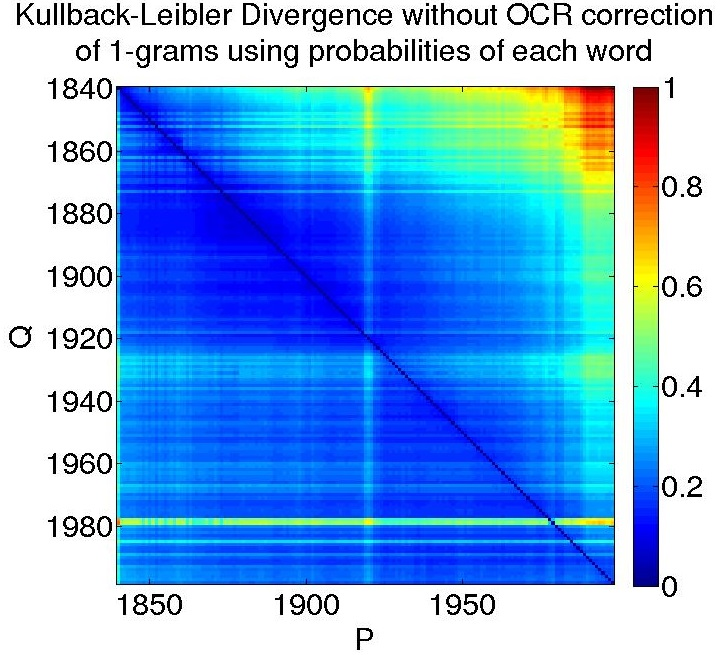
\includegraphics[scale=0.15]{Pictures/kullback-leibler/KL_1-grams_without_correction_proba.jpg}
        \caption{KL for 1-gram without OCR correction and probability of word}
        \label{}
    \end{minipage}\hfill
\end{figure}

\begin{figure}[h!]
    \begin{minipage}[b]{0.48\linewidth}
        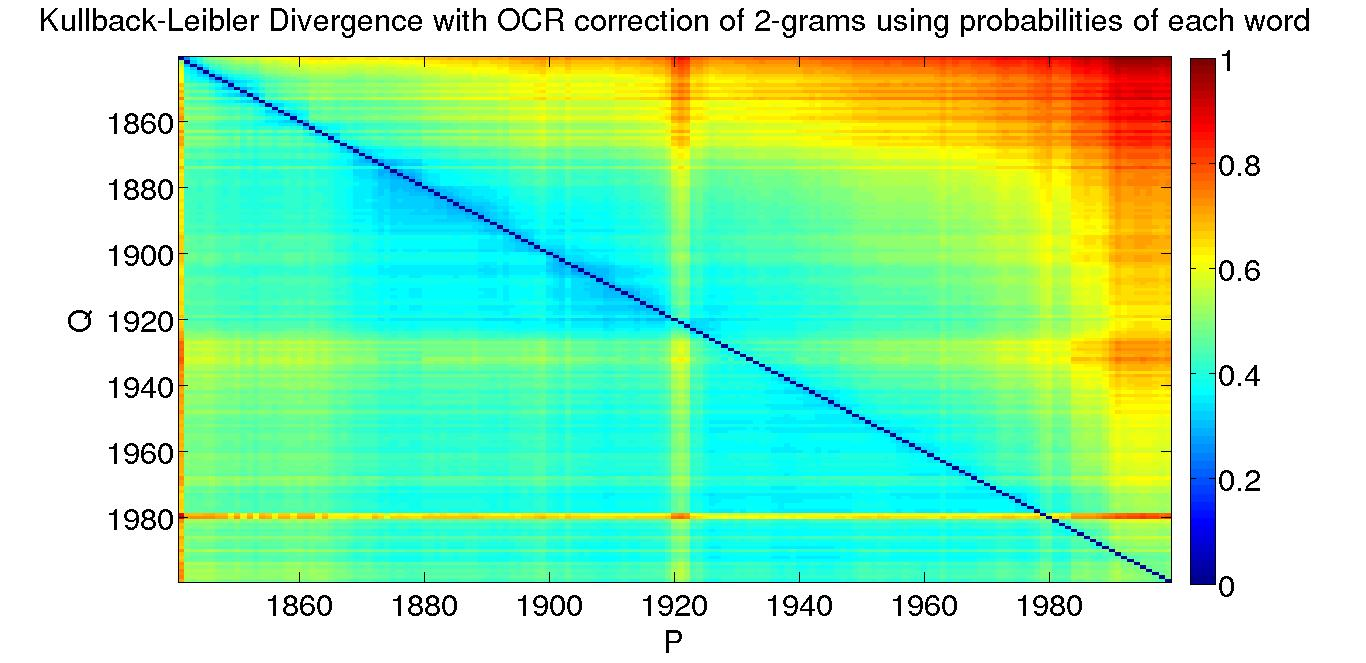
\includegraphics[scale=0.15]{Pictures/kullback-leibler/KL_2-grams_with_correction_proba.jpg}
        \caption{KL for 2-grams with OCR correction and probability of word}
        \label{}
    \end{minipage}\hfill
    \begin{minipage}[b]{0.5\linewidth}
        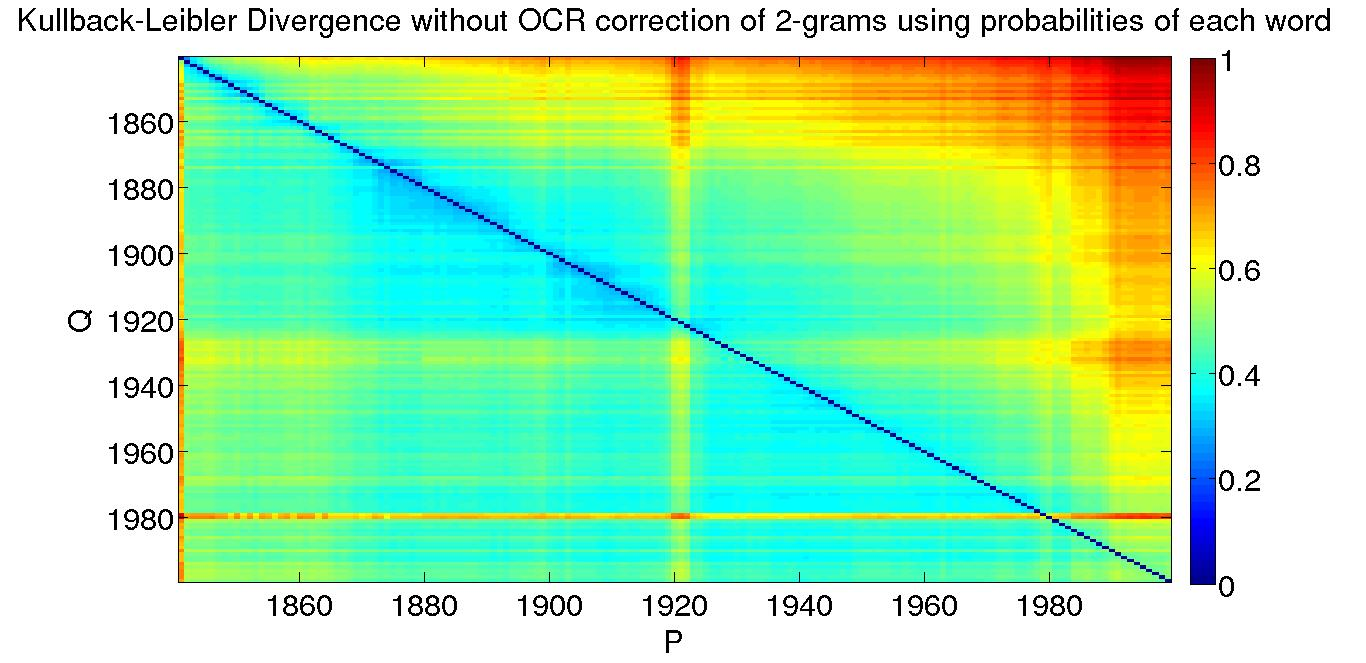
\includegraphics[scale=0.15]{Pictures/kullback-leibler/KL_2-grams_without_correction_proba.jpg}
        \caption{KL for 2-grams without OCR correction and probability of word}
        \label{}
    \end{minipage}\hfill
\end{figure}

\begin{figure}[h!]
    \begin{minipage}[b]{0.48\linewidth}
        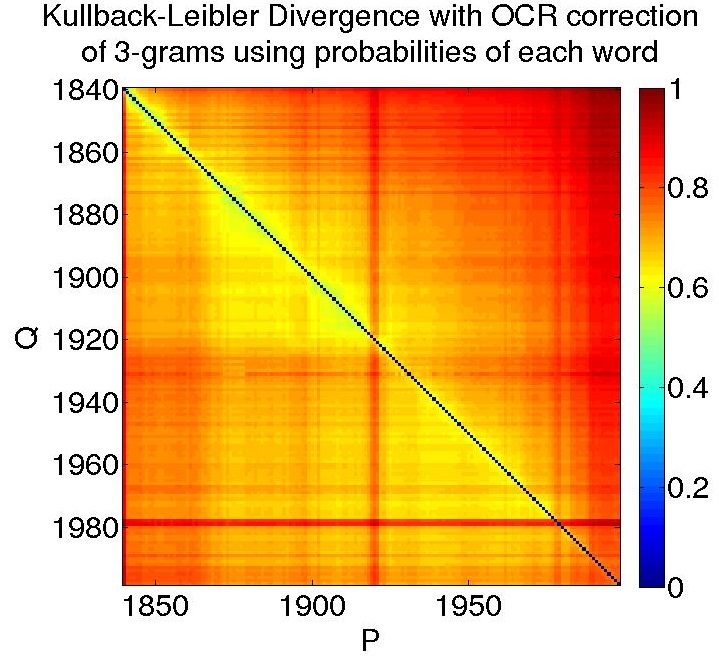
\includegraphics[scale=0.15]{Pictures/kullback-leibler/KL_3-grams_with_correction_proba.jpg}
        \caption{KL for 3-grams with OCR correction and probability of word}
        \label{}
    \end{minipage}\hfill
    \begin{minipage}[b]{0.5\linewidth}
        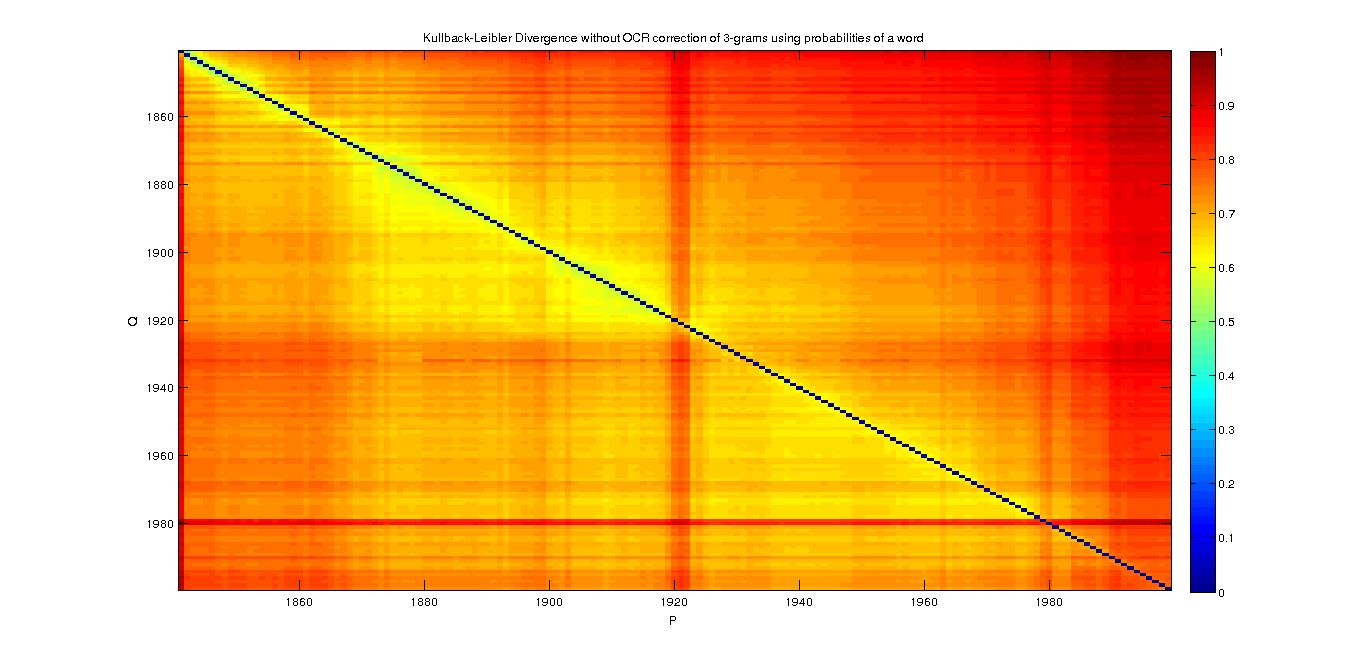
\includegraphics[scale=0.15]{Pictures/kullback-leibler/KL_3-grams_without_correction_proba.jpg}
        \caption{KL for 3-grams without OCR correction and probability of word}
        \label{}
    \end{minipage}\hfill
\end{figure}

\begin{figure}[h!]
    \begin{minipage}[b]{0.48\linewidth}
        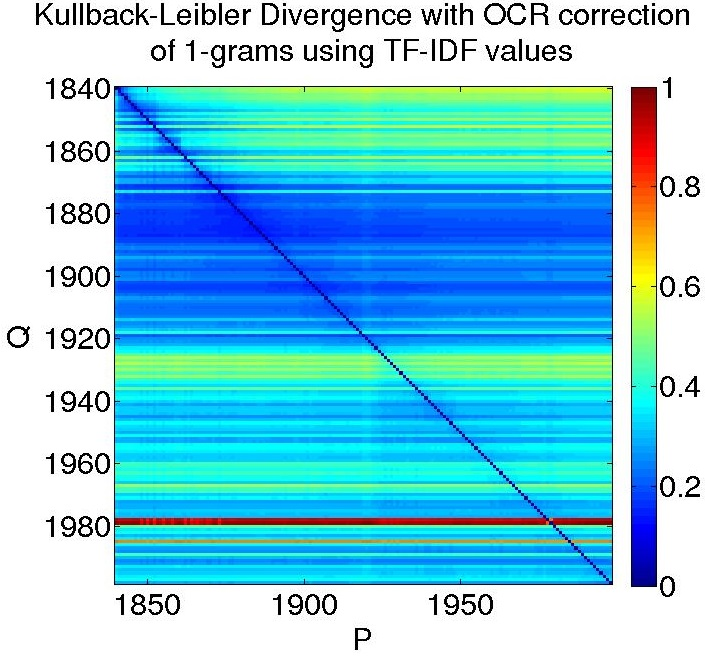
\includegraphics[scale=0.15]{Pictures/kullback-leibler/KL_1-grams_with_correction_tfidf.jpg}
        \caption{KL for 1-gram with OCR correction and TF-IDF}
        \label{}
    \end{minipage}\hfill
    \begin{minipage}[b]{0.5\linewidth}
        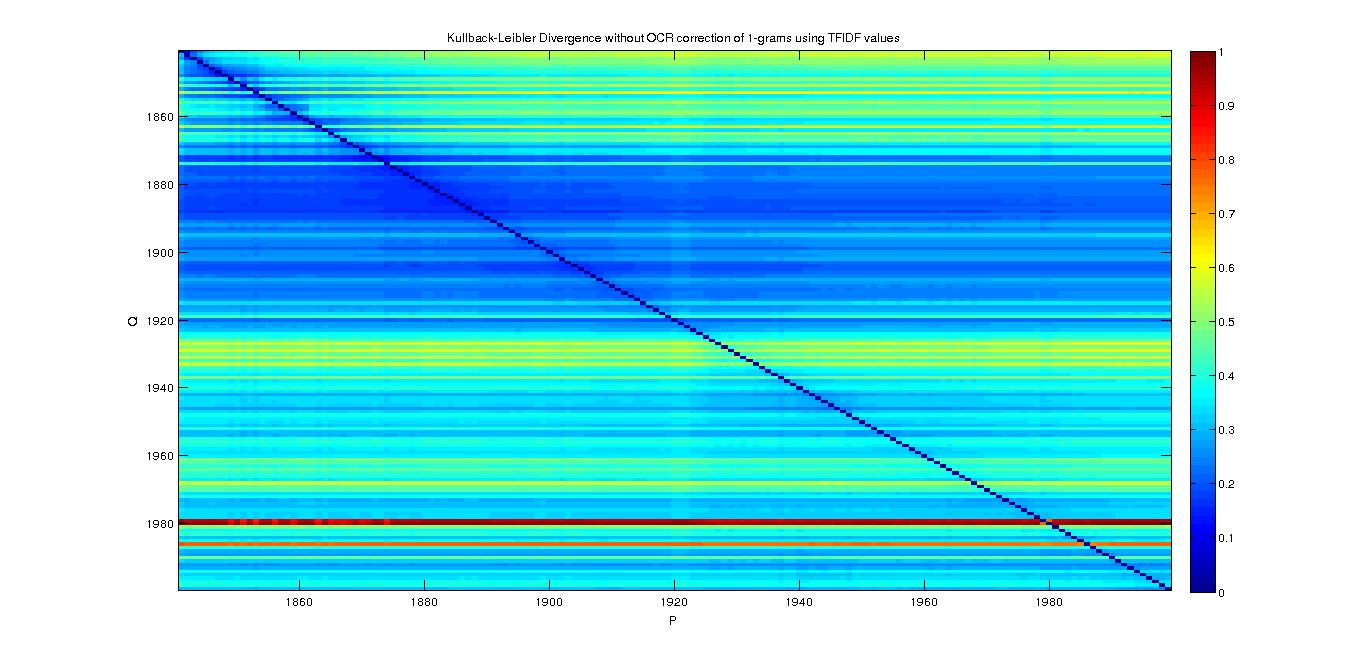
\includegraphics[scale=0.15]{Pictures/kullback-leibler/KL_1-grams_without_correction_tfidf.jpg}
        \caption{KL for 1-gram without OCR correction and TF-IDF}
        \label{}
    \end{minipage}\hfill
\end{figure}

\begin{figure}[h!]
    \begin{minipage}[b]{0.48\linewidth}
        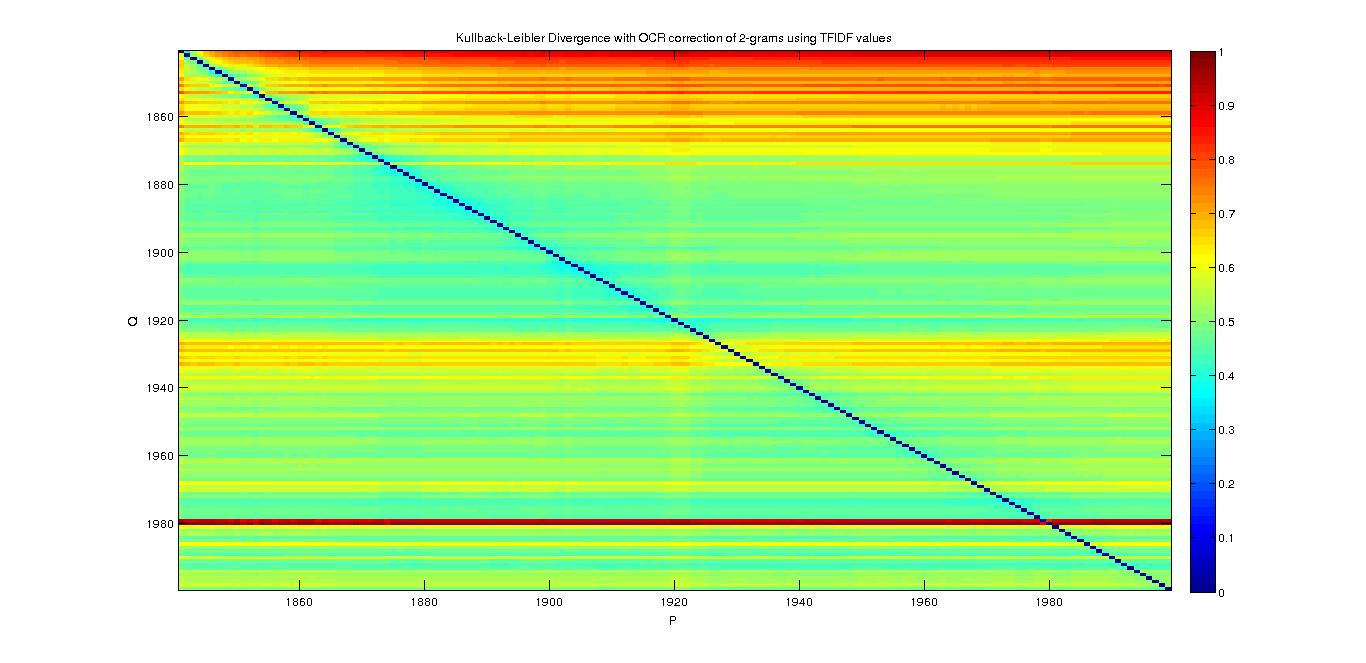
\includegraphics[scale=0.15]{Pictures/kullback-leibler/KL_2-grams_with_correction_tfidf.jpg}
        \caption{KL for 2-grams with OCR correction and TF-IDF}
        \label{}
    \end{minipage}\hfill
    \begin{minipage}[b]{0.5\linewidth}
        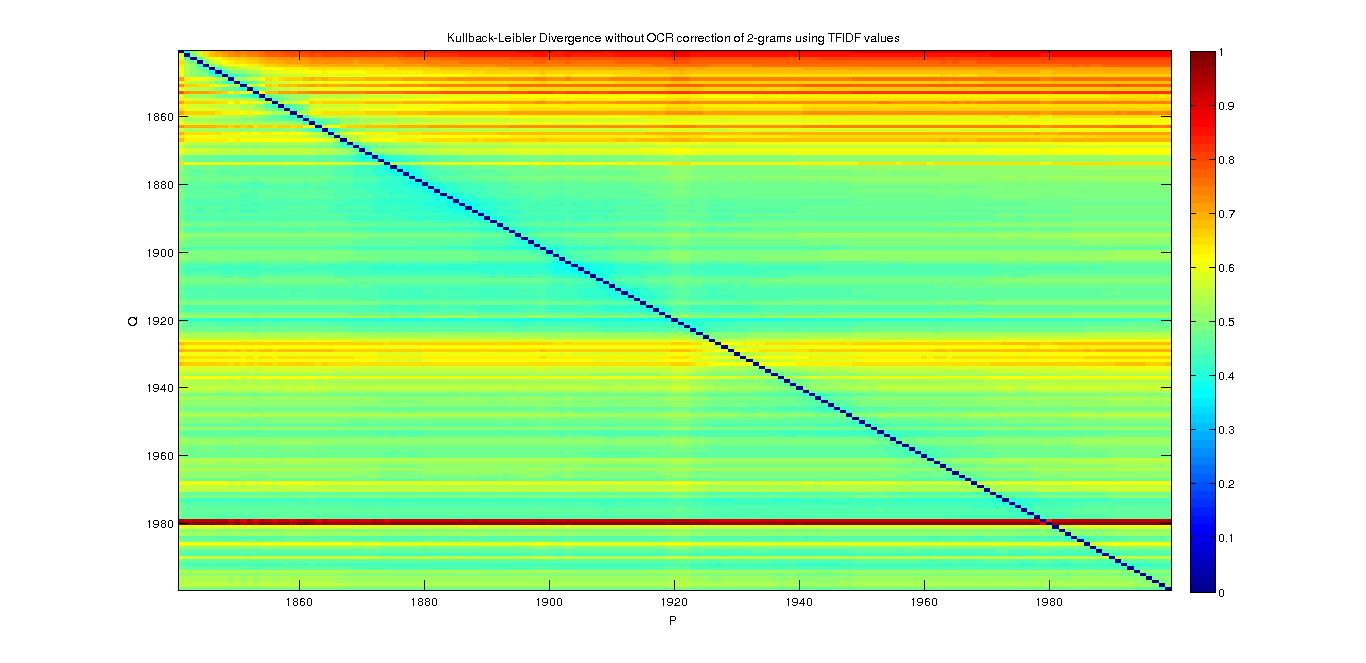
\includegraphics[scale=0.15]{Pictures/kullback-leibler/KL_2-grams_without_correction_tfidf.jpg}
        \caption{KL for 2-grams without OCR correction and TF-IDF}
        \label{}
    \end{minipage}\hfill
\end{figure}

\begin{figure}[h!]
    \begin{minipage}[b]{0.48\linewidth}
        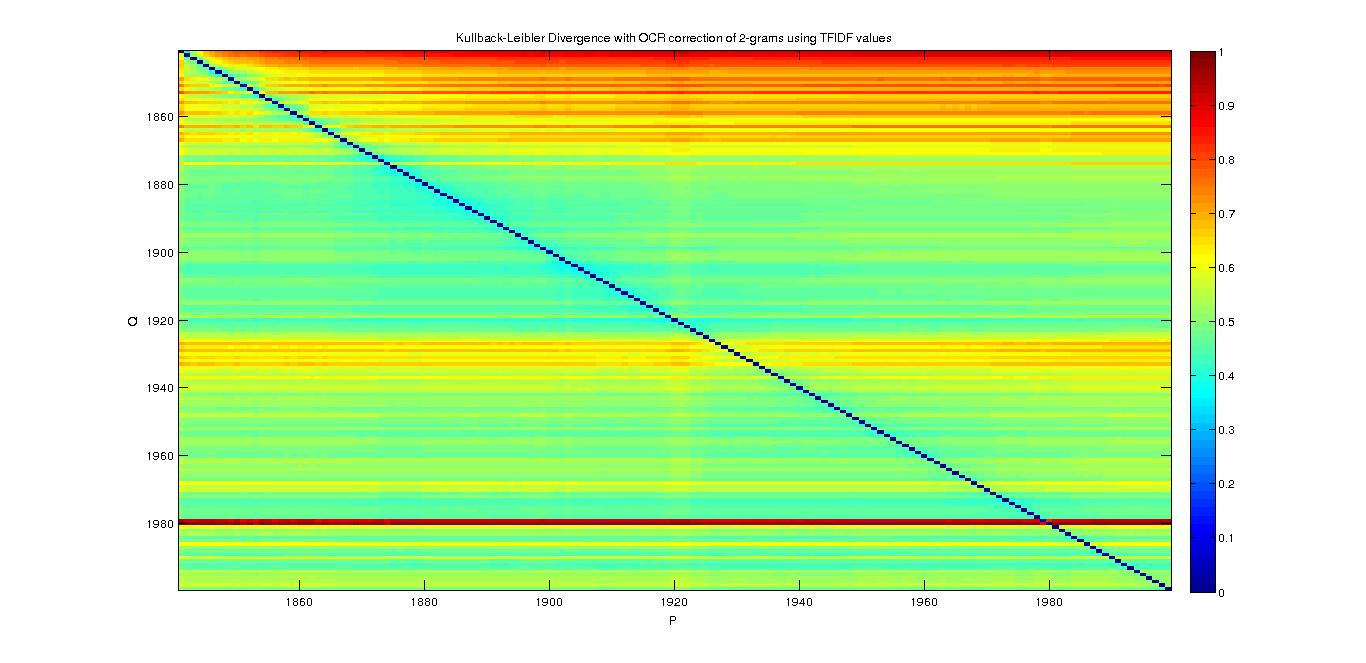
\includegraphics[scale=0.15]{Pictures/kullback-leibler/KL_2-grams_with_correction_tfidf.jpg}
        \caption{KL for 3-grams with OCR correction and TF-IDF}
        \label{}
    \end{minipage}\hfill
    \begin{minipage}[b]{0.5\linewidth}
        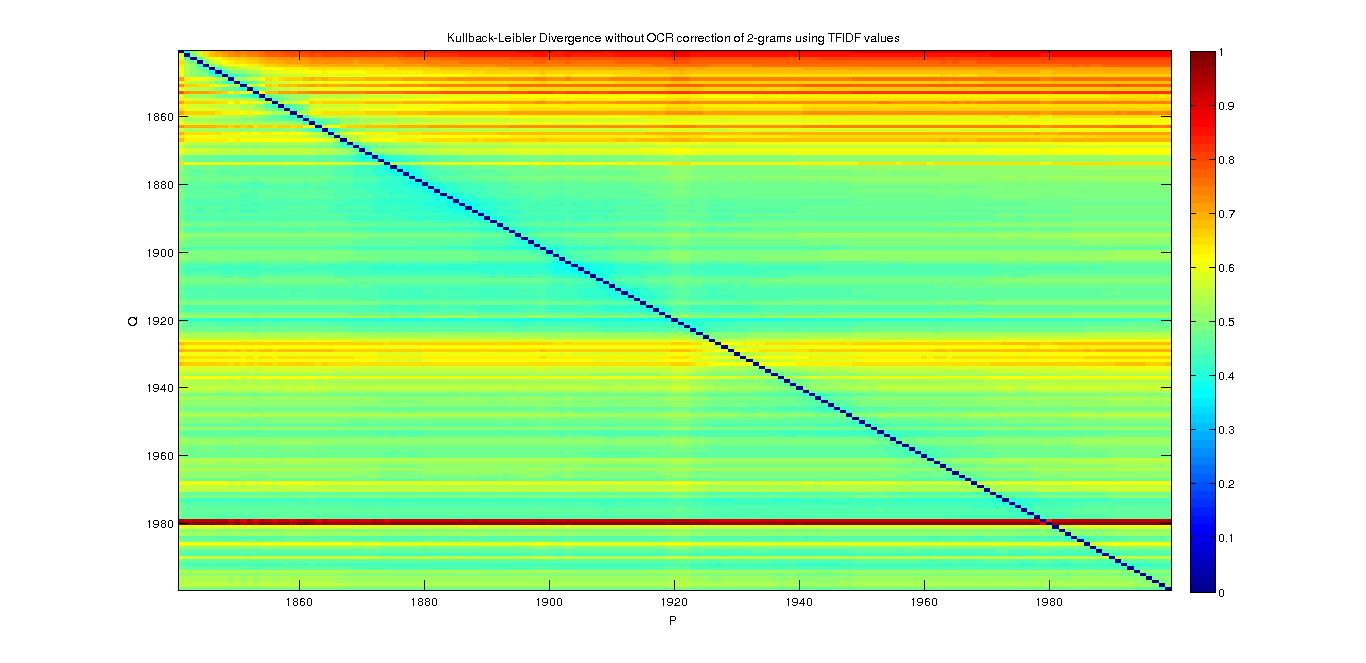
\includegraphics[scale=0.15]{Pictures/kullback-leibler/KL_2-grams_without_correction_tfidf.jpg}
        \caption{KL for 3-grams without OCR correction and TF-IDF}
        \label{}
    \end{minipage}\hfill
\end{figure}

\newpage{}

\subsubsection{Analysis of results}
Here will be the analysis